\section{Sequential Exploration: Explore Early, Exploit Late}
\label{sec:exploitation-vs-exploration}
\begin{figure}[t]
    \centering
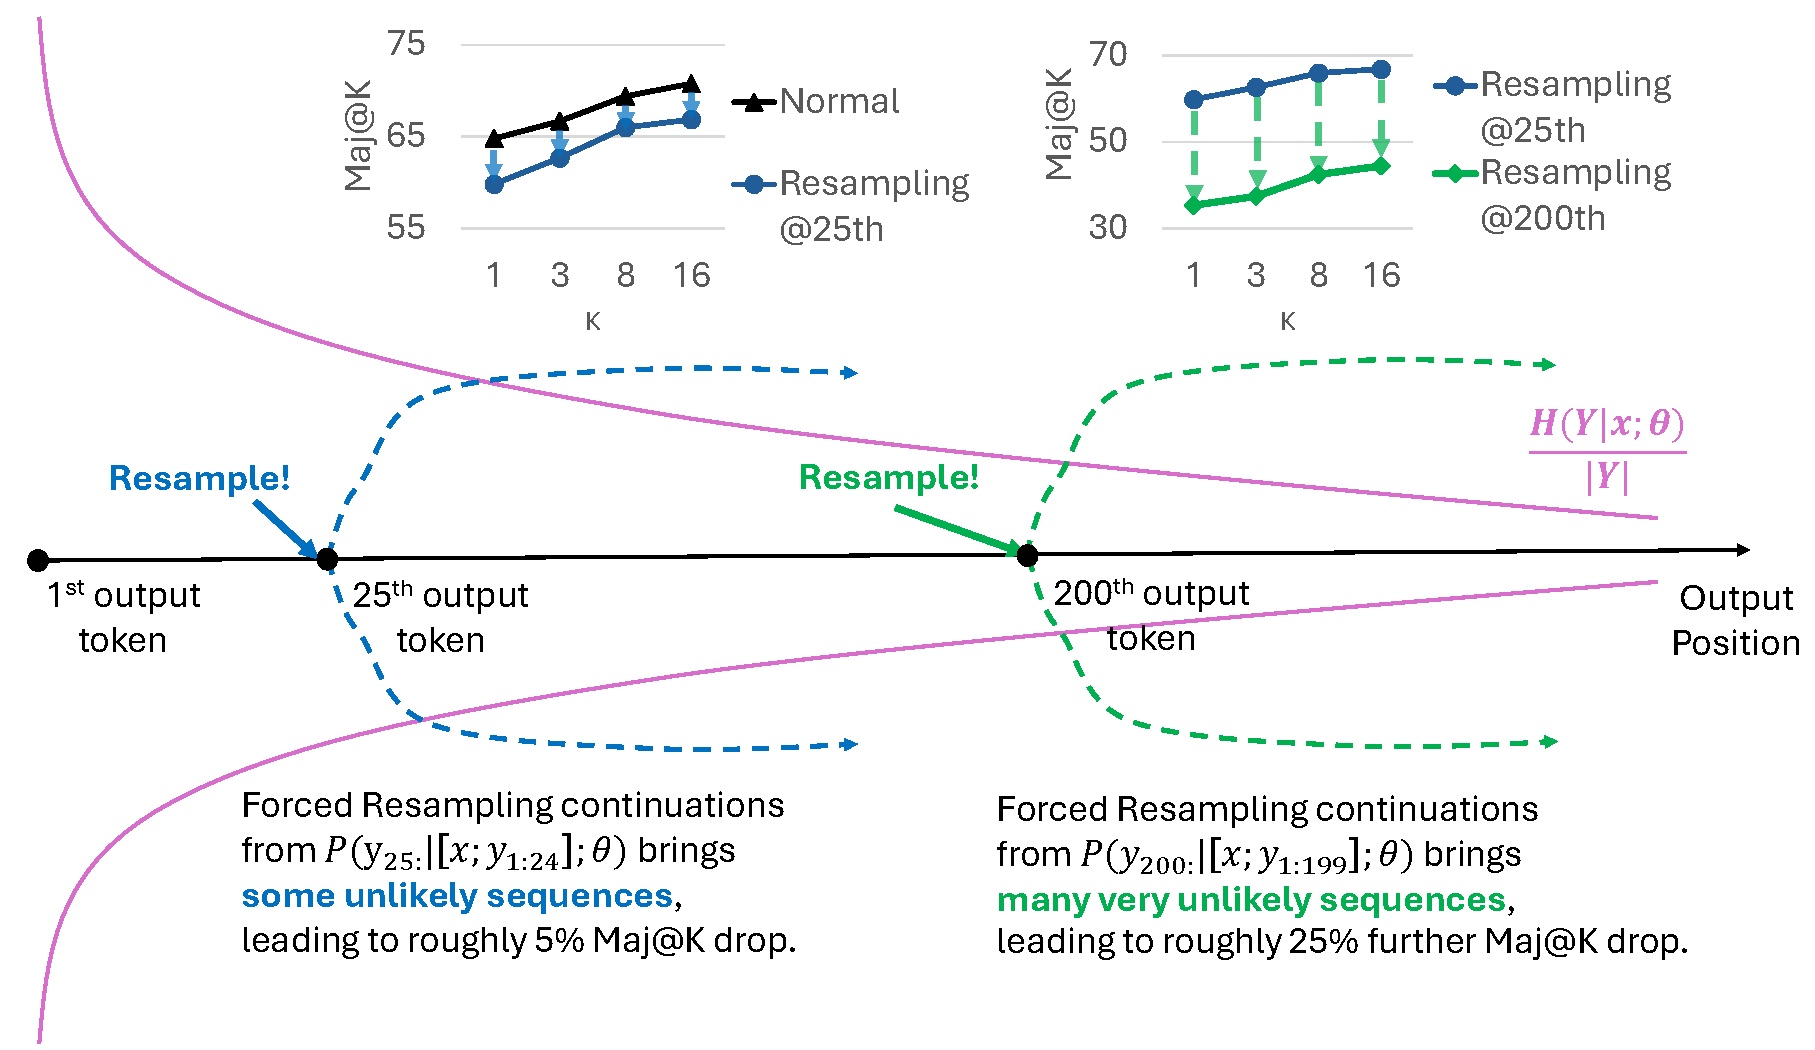
\includegraphics[width=0.9\linewidth]{icml2026/figures/branching_factor_figure/bon_from_middle_demo_v2.pdf}
% \vspace{-0.05in}
    \caption{
       A ``forking'' experiment on DeepSeek-Llama-3 shows early branching (high-entropy region) yields higher Maj@$k$ on MMLU than late branching (low-entropy region).
    }
    \vspace{-0.25in}
\label{fig:forking_experiment}
\end{figure}
%
Exploration is a cornerstone of reinforcement learning, enabling agents to discover high-quality policies rather than settling on suboptimal solutions~\citep{sutton1998reinforcement, ladosz2022exploration}. 
%
This principle becomes particularly vital in deep RL, where vast action spaces render exhaustive search infeasible.
%
In the context of RL for language models (e.g., RLVR), insufficient exploration often manifests as  \textit{entropy collapse}, i.e., a premature narrowing of the generation distribution during training~\citep{yu2025dapo, wang2025beyond, cui2025entropy}.
%  
A common simple tool to encourage exploration is \emph{temperature sampling}.
% 
However, a \textit{fixed} temperature imposes a difficult trade-off. 
%
A high temperature promotes diversity (as indicated by increased entropy\footnote{See \cref{app:entropy_proof} for the proof.}), but it risks degrading output quality with nonsensical tokens and hallucinations~\citep{renze-2024-effect, wang2025beyond}. 
%
In contrast, a low temperature limits the discovery of novel solutions, leading to generic and repetitive outputs~\citep{Holtzman2020The, guo2025deepseek}.
%
The key to resolving this dilemma lies not in finding a single best temperature, but in recognizing that exploration requirements vary throughout the generation process.
% 
This key insight stems directly from the autoregressive nature of language models.
%
At the beginning of a sequence, the context is minimal and uncertainty is high, allowing a wide range of valid continuations. 
%
As more tokens are produced, the context becomes increasingly specific, constraining subsequent choices.
%
We reference the Data Processing Inequality (DPI)~\citep{shannon1948mathematical} as a \textit{theoretical motivation} to investigate these entropy dynamics. While not a strict derivation for language  models, the DPI provides a framework to hypothesize that expected conditional entropy tends to decrease as the context grows:\footnote{While specific rollouts may have late high-entropy positions, the probability of this is exponentially small with position $t$~\citep{yang2025alignment}, making the overall trend a reliable heuristic.}
% \vspace{-10pt}
\vspace{-5pt}
\begin{equation}
\label{eq:entropy_decay}
\begin{split}
H(Y_t | [x, Y_{<t}]; \theta) &= \underbrace{\mathbb{E}_{y_{<t}}\big[ H(Y_t | [x, y_{<t}]; \theta) \big]}_{\substack{\text{Expected entropy at step } t \\ \text{(average over all prefixes } y_{<t}\text{)}}} \\
&\geq 
\underbrace{\mathbb{E}_{y_{<t+1}}\big[ H(Y_{t+1} | [x, y_{<t+1}]; \theta) \big]}_{\substack{\text{Expected entropy at step } t+1 \\ \text{(average over all prefixes } y_{<t+1}\text{)}}} \\
&= H(Y_{t+1} | [x, Y_{<t+1}]; \theta)\nonumber 
\end{split}
\end{equation}

\vspace{-10pt}

\begin{figure}[t]
    \centering
    \includegraphics[width=0.8\linewidth]{icml2026/figures/annealing_schedule_plot.pdf}
    \caption{
     The annealing schedule with different decay rates $d$. A larger $d$ slows the cooling, front-loading exploration over more tokens. We set $c=10, \tau_{\mathrm{max}}=1.2, \tau_{\mathrm{min}}=0.1$ for illustration.
    }
    \label{fig: annealing_schedule_demo}
    \vspace{-20pt}
\end{figure}
\cref{fig: entropy_sequential_dynamic} presents an empirical validation,  examining position-wise entropy trend on MMLU ~\citep{hendrycks2021measuring}\footnote{We use MMLU as a held-out dataset with Chain-of-Thought prompting~\citep{wei2022chain} to incentivize longer reasoning outputs, aligning with a typical RLVR scenario.} with Llama-3-8B-Instruct~\citep{grattafiori2024llama}.

This entropy decay has a direct performance implication: effective exploration, producing diverse, high-quality responses, is most beneficial in an uncertain, high-entropy phase at the start of generation.
%
To verify this, we replicate a controlled ``forking'' experiment~\citep{yang2025alignment} on DeepSeek-Distilled Llama-3-8B~\citep{guo2025deepseek}, a representative RLVR-fine-tuned model from the same Llama-3 family. 
%
As shown in \cref{fig:forking_experiment}, trajectories branched from early generation steps consistently outperform those branched later. 
%
% YCH: "align/aligning" should not occur that often in the near context -- it is again stylistically weak.  
This finding is also consistent with observations from inference-time analysis, where forced, late-stage exploration tends to degrade output quality~\citep{liao2025lost, yang2025alignment, fu2025deep}.
%

% I think mentioning classic results is redundant here.
% These converging lines of evidence provide a clear guide for applying a classic RL principle: agents should increase exploration in states of high uncertainty~\citep{ziebart2008maximum, schulman2017equivalence, haarnoja2018soft}. 
%
Aligning our strategy with the natural dynamics of generation, we arrive at a simple yet powerful design principle: \textbf{explore early and exploit late}.

%

% This position-dependent entropy curve provides a clear guide for applying a classic RL principle: agents should increase exploration in states of high uncertainty~\citep{ziebart2008maximum, schulman2017equivalence, haarnoja2018soft}. 
% %
% By aligning our strategy with the natural dynamics of generation, we arrive at a simple yet powerful design principle: \textbf{explore early and exploit late}. 
% %
% This involves encouraging strong exploration when the generative trajectory is wide, and gradually shifting toward exploitation as it narrows. 
% %
% In the next section, we will introduce a concrete method that instantiates this principle.
%
% The key to resolving this dilemma lies not in finding a single best temperature, but in recognizing that the need for exploration changes throughout the generation process. This insight stems directly from the autoregressive nature of language models, where the expected conditional entropy tends to decrease with each step (see \cref{eq:entropy_decay}). We empirically demonstrate that this entropy decay is a robust phenomenon across different types of models in \cref{fig:entropy_comparison}. The trend holds for a general-purpose instruct model (\cref{fig:entropy_instruct}) and is equally prominent in a state-of-the-art reasoning model fine-tuned with RLVR-style distillation (\cref{fig:entropy_rlvr}).

% \section{Sequential Exploration: Explore Early, Exploit Late}
% \label{sec:exploitation-vs-exploration}
% Exploration is a cornerstone of RL, enabling agents to discover effective policies and avoid converging to suboptimal solutions~\citep{sutton1998reinforcement, ladosz2022exploration}. This principle is especially critical in deep RL, where vast action spaces make exhaustive search intractable. In the context of RLVR, insufficient exploration often manifests as \textit{entropy collapse}---a premature narrowing of the generation distribution~\citep{yu2025dapo, wang2025beyond, cui2025entropy}. A common tool to encourage exploration is temperature sampling; however, a \textit{fixed} temperature imposes a difficult trade-off. A high temperature promotes diversity but risks introducing nonsensical outputs late in the generation process~\citep{renze-2024-effect, wang2025beyond}, while a low temperature limits the discovery of novel solutions~\citep{Holtzman2020The, guo2025deepseek}.

% The key to resolving this dilemma lies not in finding a single best temperature, but in recognizing that the need for exploration changes throughout the generation process. This insight stems directly from the autoregressive nature of language models. At the beginning of a sequence, the context is minimal and uncertainty is high. As the model generates more tokens, the context becomes increasingly specific, constraining future choices. This natural uncertainty reduction is formalized by the data processing inequality, which shows that expected conditional entropy tends to decrease with each step:\footnote{While specific rollouts may have late high-entropy positions, the probability of this will decay quickly with position $t$~\citep{yang2025alignment}, making the overall trend a reliable heuristic.}
% \begin{equation}
% \label{eq:entropy_decay}
% H(Y_t | [x, Y_{<t}]) = \underbrace{\mathbb{E}_{y_{<t}}\big[ H(Y_t | [x, y_{<t}]) \big]}_{\substack{\text{Expected entropy at step } t}}
% \geq 
% \underbrace{\mathbb{E}_{y_{<t+1}}\big[ H(Y_{t+1} | [x, y_{<t+1}]) \big]}_{\substack{\text{Expected entropy at step } t+1}} = H(Y_{t+1} | [x, Y_{<t+1}])\nonumber
% \end{equation}
% \begin{wrapfigure}{r}{0.45\textwidth}
% \vspace{-0.15in}
%     \centering
%     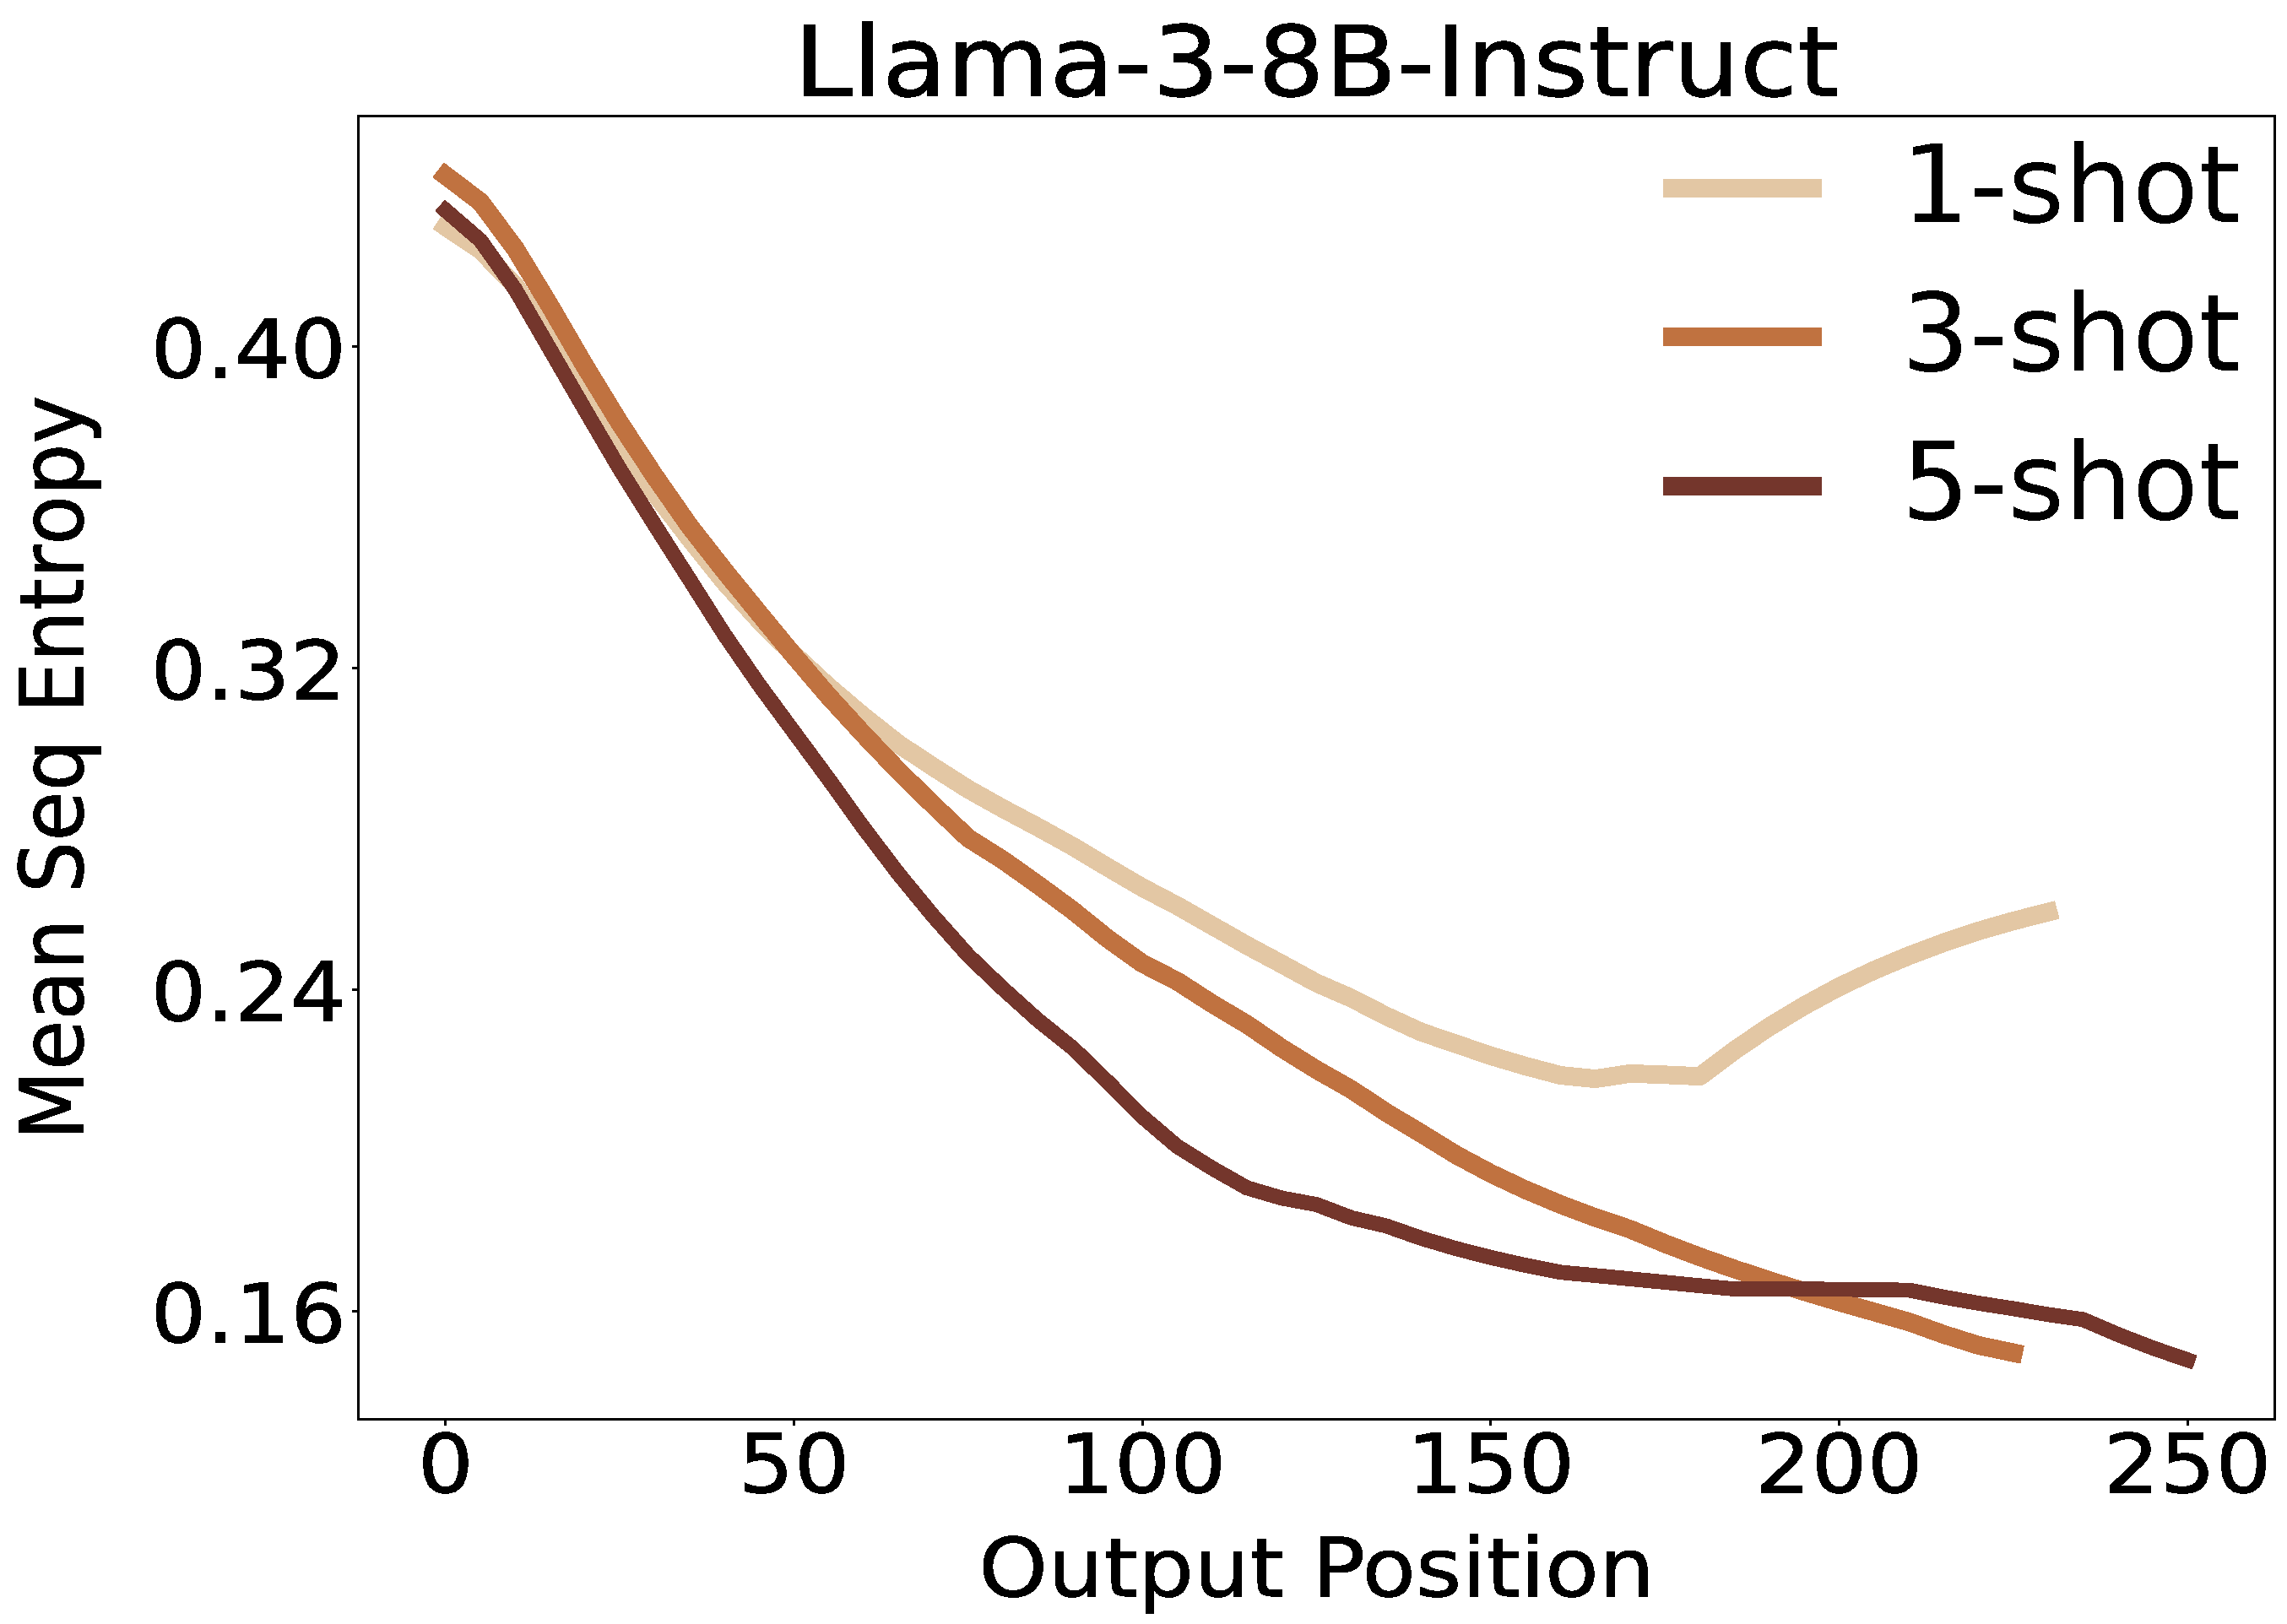
\includegraphics[width=\linewidth]{iclr2026/figures/branching_factor_figure/piecewise_ebf_Llama-3-8B-Instruct_mean_seq_entropy_fixed_start.pdf}
%     \vspace{-5mm}
%     \caption{
%     Entropy dynamics for Llama-3-8B-Instruct on the MMLU dataset. }
%     \vspace{-0.05in}
%     \label{fig: entropy_sequential_dynamic}
% \end{wrapfigure}
% We empirically validate this position-wise entropy trend on the MMLU dataset~\citep{hendrycks2021measuring}\footnote{We use MMLU as a held-out dataset with Chain-of-Thought prompting~\citep{wei2022chain} to incentivize longer reasoning outputs, aligning with a typical RLVR scenario.} using Llama-3-8B-Instruct~\citep{grattafiori2024llama}, as illustrated in \cref{fig: entropy_sequential_dynamic}.

% This trend is not merely an artifact of RL training but reflects a fundamental property known as \textit{LLM probability concentration}, where the next-token distribution naturally sharpens as generation progresses~\citep{yang2025alignment}. Indeed, research on inference-time decoding has similarly found that forcing exploration late in the sequence degrades performance by injecting low-quality outputs~\citep{liao2025lost, fu2025deep}. The well-documented continuity between base and RL-tuned models~\citep{yue2025does, zhao2025echo} indicates this principle holds true for RLVR as well, suggesting that an effective strategy must not only explore high-entropy areas, but also fruitful ones.

% These converging lines of evidence provide a clear guide for applying a classic RL principle: agents should increase exploration in states of high uncertainty~\citep{ziebart2008maximum, schulman2017equivalence, haarnoja2018soft}. By aligning our strategy with the natural dynamics of generation, we arrive at a simple yet powerful design principle: \textbf{explore early and exploit late}. This involves encouraging strong exploration when the generative trajectory is wide and gradually shifting toward exploitation as it narrows. In the next section, we will introduce a concrete method that instantiates this principle.